\documentclass[a4paper]{article}
\usepackage[utf8]{inputenc}
\usepackage[russian,english]{babel}
\usepackage[T2A]{fontenc}
\usepackage[left=10mm, top=20mm, right=18mm, bottom=15mm, footskip=10mm]{geometry}
\usepackage{indentfirst}
\usepackage{amsmath,amssymb}
\usepackage[italicdiff]{physics}
\usepackage{graphicx}
\graphicspath{{images/}}
\DeclareGraphicsExtensions{.pdf,.png,.jpg}
\usepackage{wrapfig}

\usepackage{caption}
\captionsetup[figure]{name=Рисунок}
\captionsetup[table]{name=Таблица}
  
\title{\underline{Отчет о выполненой лабораторной работе 1.4.2}}
\author{Воронин Денис, Б04-403}

\begin{document}
\maketitle
\begin{center}
    \textbf{ОПРЕДЕЛЕНИЕ УСКОРЕНИЯ СВОБОДНОГО ПАДЕНИЯ ПРИ ПОМОЩИ ОБОРОТНОГО МАЯТНИКА}
\end{center}

\section{Аннотация}
\textbf{Цель работы:}с помощью оборотного маятника измерить величину ускорения свободного падения.

\textbf{В работе используются:}оборотный маятник с двумя подвесными призмами и 
двумя грузами (чечевицами); электронный счётчик времени и числа колебаний;
подставка с острием для определения положения центра масс маятника; закреплённая на стене консоль для подвешивания маятника; металлические линейки, штангенциркуль длиной 1 м.

\section{Теоретические сведения}
Физическим маятником называют твёрдое тело, способное совершать 
колебания в вертикальной плоскости, будучи подвешено за одну из своих 
точек в поле тяжести. Ось, проходящая через точку подвес перпендикулярно плоскости качания, называется осью качания маятника.\par
При малых колебаниях период колебаний физического маятника определяется формулой (1): \[T = 2\pi \sqrt{\frac{J}{mgl} } \] \par
Где J — момент инерции маятника относительно оси качания, m — масса 
маятника, l — расстояние от оси качания до центра масс маятника.\par
Если сравнить (1) c известной формулой колебаний математического 
маятника длиной ${l_{m}}$ \[T = 2\pi \sqrt{\frac{{l_{m}}}{g} }\] , можно определить приведённую длину физического маятника как (4)
\[l_{\text{пр}}=\frac{J}{ml}\]\par

Смысл приведённой длины в том, что при длине математического маятника, равной ${l_{m}}$ = $l_{\text{пр}}$ , его период колебаний совпадает с периодом колебаний данного физического маятника.

\section{Теорема Гюйгенса об оборотном маятнике}

\begin{figure}[h]
    \centering
    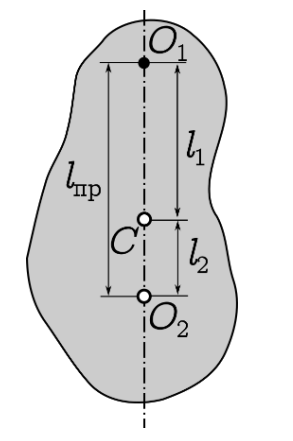
\includegraphics[width=0.2\textwidth]{pick1.PNG} 
    \caption{К теореме Гюйгенса}
    \end{figure}
    Докажем теорему Гюйгенса об оборотном маятнике. 
Пусть ${O_{1}}$ и ${O_{2}}$ — две точки подвеса физического маятника, лежащие на одной прямой с точкой C по разные стороны от неё (см.рис.1). Тогда периоды колебаний маятника равны соответственно(5)
\[T_{1} = 2\pi \sqrt{\frac{J_{1}}{mgl_{1}} },  T_{2} = 2\pi \sqrt{\frac{J_{2}}{mgl_{2}} } \] 

По теореме Гюйгенса—Штейнера имеем (2):
\[J_{1} = J_{C}+ml^{2}_{1},  J_{2} = J_{C}+ml^{2}_{2} \]
где $J_{C}$ — момент инерции маятника относительно оси, проходящей через 
центр масс перпендикулярно плоскости качания.
Пусть периоды колебаний одинаковы: $T_{1}$ =$T_{2}$. Тогда одинаковы 
должны быть и приведённые длины: \[l_{\text{пр}} = \frac{J_{1}}{ml_{1}}=\frac{J_{2}}{ml_{2}} \]

С учетом (2) получим (8): \[l_{\text{пр}} = \frac{J_{C}}{ml_{1}}+l_{1}=\frac{J_{C}}{ml_{2}}+l_{2} \]
откуда находим (при $l_{2} \neq l_{1}$)
\[J_{C} = ml_{1}l_{2}\]
Подставляя обратно получим (3)
$l_{\text{пр}}=l_{1}+l_{2}$
Таким образом, доказано следующее: если периоды колебаний при подвешивании маятника в точках $O_{1}$ и $O_{2}$ равны, то расстояние между точками 
подвеса равно приведённой длине маятника; и наоборот, из равенства (3)
следует равенство периодов $T_{1} = T_{2}$.


\section{Измерение g}
Пусть \[L \equiv \overline{O_{1}O_{2}}  = l_{1} + l_{2}\] — расстояние между двумя «сопряжёнными» 
точками подвеса физического маятника. Если соответствующие периоды 
малых колебаний равны, $T_{1}=T_{2}=T$, то по теореме Гюйгенса L = ${l_\text{пр}}$. Тогда из (1) и (4) находим ускорение свободного падения (6)
\[g_{0}=(2\pi)^2\frac{L}{T^2}\]
Точного совпадения $T_{1}=T_{2}$ на опыте добиться, конечно, невозможно. 
Поэтому получим формулу для определения ускорения свободного падения g, если измеренные периоды незначительно различаются:
\[T_{1}=T, T_{2}=T+\vartriangle T\]
Из системы (5) и (2) получаем(7):
\[g=(2\pi )^2\frac{l_{1}^2-l_{2}^2}{T_{1}^2l_{1}-T_{2}^2l_{2}}\]
Можно переписать (7) как:
\[g=g_{0}\frac{\lambda-1}{\lambda - \frac{T_{2}^2}{T_{1}^2} }, \text{где} \lambda = \frac{l_{1}}{l_{2}}\]
Проанализируем отличия формулы (7) от (6) и оценим величину поправки. Пусть $\varepsilon = \frac{\vartriangle T}{T}\ll 1 $
— относительное отклонение при измерении периодов. Тогда при $\lambda\neq 1$, пользуясь малостью $\varepsilon$ , получим (9)
\[g = g_{0}\frac{\lambda -1}{\lambda -(1+\varepsilon )^2}\approx g_{0}\frac{1}{1-\frac{2\varepsilon }{\lambda -1} }\approx g_{0}(1+\frac{2\varepsilon }{\lambda -1} )\]  


\section{Экспериментальная установка}
В работе используются маятники в форме стержней цилиндрического
или прямоугольного сечения длиной $\thicksim 1$ м и массой $1/1.5$ кг. Маятник 
подвешивается с помощью небольших треугольных призм ($\text{П}_{1} \text{и} \text{П}_{2}$), острым основанием опирающихся на закреплённую на стене консоль. Ребро 
призмы задаёт ось качания маятника. На стержне закрепляются два дополнительных груза в форме «чечевицы»($\text{Г}_{1} \text{и} \text{Г}_{2}$). Для выполнения условия 
$l_{1}>l_{2}$ внешнюю чечевицу $\text{Г}_{2}$ следует крепить за призмой $\text{П}_{2}$, а чечевицу $\text{Г}_{1}$
(внутреннюю) — между призмами $\text{П}_{1} \text{и} \text{П}_{2}$ (см. Рис. 3).\par
Регистрация времени колебаний проводится с помощью электронных 
счётчиков. Расстояния между точками установки маятников на консоли до 
электронных счётчиков фиксировано. Это накладывает ограничения на расположение призм и грузов на стержне. Призмы крепятся симметрично
на равном расстоянии от концов стержней так, чтобы маятник при колебаниях пересекал фотоприёмники счётчика, не задевая оправу счётчика. 

\begin{figure}[h]
    \centering
    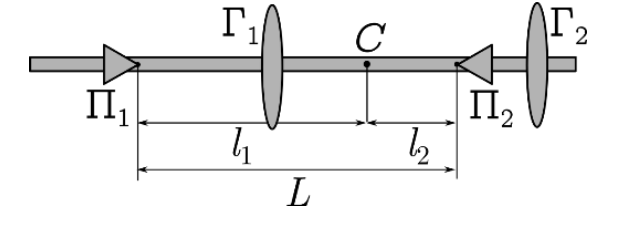
\includegraphics[width=0.5\textwidth]{pick2.PNG} 
    \caption{Маятник с грузами}
    \end{figure}

Фиксированное положение призм однозначно задаёт приведённую длину оборотного маятника $l_{\text{пр} = L }$. Изменять в опыте можно только положения грузов на стрежне. Главная задача опыта — подобрать такое положение грузов, при котором периоды колебаний при перевороте маятника 
совпадали бы с достаточно высокой точностью, а для положения центра 
масс маятника выполнялось при этом условие $\frac{l_{1}}{l_{2}}>1,5 $.

\section{Предварительный расчёт положения грузов}
Если первоначально расположить грузы на стержне произвольным образом, то для достижения равенства периодов колебаний потребуется исследовать зависимости периодов колебаний $T_{1} \text{и} T_{2}$ при перемещении поочерёдно обоих грузов по штанге.\par
Существенно облегчить и ускорить поиск нужного положения грузов 
можно, если провести предварительные расчёты.После установки грузов согласно предварительным расчёам, их положение может быть уже уточнено экспериментально.\par
Пусть призмы $\text{П}_{1} \text{и} \text{П}_{2}$ задают сопряжённые точки подвеса, то есть период колебаний при перевороте маятника не изменяется. Тогда по теореме 
Гюйгенса расстояние между призмами L — это приведённая длина маятника. Это условие может быть записано либо в форме (4)
\[J_{\text{пр}}= MLl_{2}\]
где $J_{\text{п}}$ — момент инерции маятника относительно призмы $\text{П}_{2}$ , либо в 
форме (8):
\[J_{C} = Ml_{1}l_{2}\]
где $J_{C}$ — момент инерции маятника относительно его центра масс. Здесь 
M — полная масса маятника.

\section{Оценка погрешностей}
Оценим влияние погрешностей измерений на точность расчётов по формуле (7). Пусть все периоды измерены с одинаковой погрешностью $\sigma_{T}$, 
расстояние L между точками подвеса с погрешностью $\sigma_{L}$, расстояния $l_{1,2}$
до центра масс с погрешностью $\sigma_{l}$. Погрешность определения величины $g_{0}$
(по формуле (6)) равна
\[\frac{\sigma_{g0}}{g_{0}}=\sqrt{(\frac{\sigma_{l}}{L} )^2+4(\frac{\sigma_{T} }{T} )^2}\]
Это — основная погрешность опыта. Видно, что для её минимизации необходимо максимально точно измерить расстояние между точками повеса L
и период колебаний маятника T.
Проанализируем влияние поправки $g= g_{0}+\bigtriangleup g$, где согласно (9)  
\[\bigtriangleup g\approx 2\beta \frac{\bigtriangleup T}{T}g_{0}, \beta \frac{l_{2}}{l_{1}-l_{2}}\] 
Общая формула для погрешности (7) слишком громоздка, поэтому для 
наглядности анализа проведём вычисления приближённо. Достаточно учесть, что основной вклад в относительную погрешность $\bigtriangleup g$ вносят величины $\bigtriangleup T \text{и} \bigtriangleup l = l_{1}-l_{2}$ , поскольку являются разностями двух близких величин.
Тогда для полной относительной погрешности получим(10)
\[\frac{ \sigma_{g}}{g}\thickapprox \sqrt{(\frac{\sigma_{L}}{L} )^2+ 4(1+2\beta)(\frac{\sigma T}{T} )^2+8(\beta \frac{\bigtriangleup T}{T}\frac{\sigma_{l}}{\bigtriangleup l})^2}\]

\section{{Ход работы}}
\subsection{Измерение масс}

\begin{table}[!h]
    \begin{center}
    \begin{tabular}{|l|l|}
    \hline
    Элемент & m,г \\ \hline
    Целиком                        & 4023$\pm 0,1$                      \\ \hline
    Стержня                        & 891,5$\pm 0,1$                    \\ \hline
    Груз 1                        & 1495,5 $\pm 0,1$                    \\ \hline
    Груз 2                        & 1481,3 $\pm 0,1$                    \\ \hline
    Призма 2                        & 76,6 $\pm 0,1$                    \\ \hline
    Призма 1                        & 78,3 $\pm 0,1$                     \\ \hline
    \end{tabular}
    \caption{Масса маятника стержня груза и призм}
    \end{center}
    \end{table}

\subsection{Измерение длины}
Расстояние между призмами: 
\[L = 50,41\pm 0,05\text{см}\]
Длина всего стержня:
\[l_{\text{ст}} = 98.31\pm 0,05\text{см}\]

\subsection{Рассчет положения грузов на стержне}
С помощью программы произведем рассчет положения грузов:
Из имеющихся данных (см.табл.1) получаем:\par
Масса маятника вычисленная(M) = 4023,2\par
\[L_{1}= 36\text{см}, \text{и} L_{2}= 14,4\text{см}, \text{при} \frac{L_{1}}{L_{2}}=2,5 \]
Момемнт инерции относительно призмы $\text{П}_{2}$:

\begin{table}[!h]
    \begin{center}
    \begin{tabular}{|l|l|}
    \hline
    Момент инерции стержня $J_{\text{ст}}$                        & 0,148 $\text{кг}*\text{м}^2$                      \\ \hline
    Момент инерции маятника J                        & 0,292 $\text{кг}*\text{м}^2$                   \\ \hline
    \end{tabular}
    \caption{}
    \end{center}
    \end{table}

По вычисленным данным построим график зависимости момента инерции от положения грузов и определим точку пересечения
\begin{figure}[h]
    \centering
    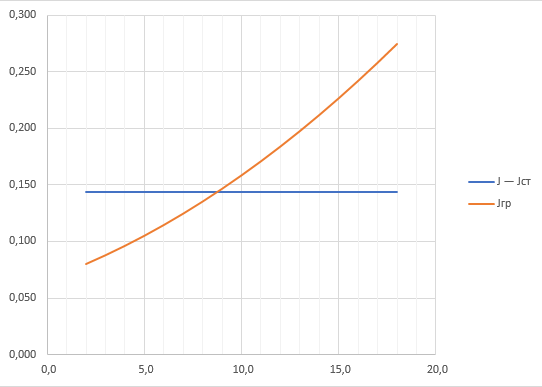
\includegraphics[width=0.35\textwidth]{pick3.PNG} 
    \caption{Зависимость момента инерции от положения грузов}
    \end{figure}

Из графика получим, что $L_{1} = 9 \text{см}$, а $L_{2} = 50,41-9=41,41 \text{см}$\par
Уточним эти значения с помощью программы: 

\begin{figure}[h]
    \centering
    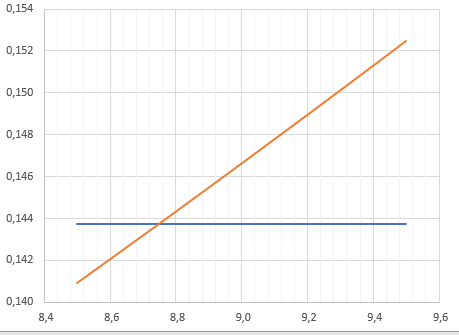
\includegraphics[width=0.35\textwidth]{pick4.PNG} 
    \caption{Уточнение положения точки пересечения}
    \end{figure}

Из графика получим, что $L_{1} = 8,8 \text{см}$, а $L_{2} = 50,41-8,8=41,61 \text{см}$\par
С помощью $\bot$ -образной подставки определите положение центра масс 
маятника с грузами. Получим 32,81\par
Измерим расстояние $l_{1} \text{и} l_{2}$: от центра масс до
острия призм  $\text{П}_{1} \text{и} \text{П}_{2} $ соответственно. Получим $l_{2} = 10,9 \text{и} l_{1} = 38,8$

\subsection{Рассчет периода колебаний }
При измерении времени для n = 10 колебаний значение $T_{2} = 14,51\pm 0,01\text{с}$\par
При подвешивании на призму $\text{П}_{1}$ период для n = 10 колебаний $T_{1} = 14,53\pm 0,01$ \par
Сравнивая значения $T_{1}\text{и} T_{2} $ получаем, что различие $\frac{\bigtriangleup T}{T}\approx 0,13\%  $, что не превышает 1\%, значит можем переходить к следующему пункту.\par
Проведем окончательное измерение периодов  $T_{1}\text{и} T_{2} $ с максимальной точностью. Количесвто колебаний выберем равным n = 20. По результатам измерений имеем следующиее:

\begin{table}[!h]
    \begin{center}
    \begin{tabular}{|l|l|l|}
    \hline
    № измерения  & $T_{\text{п1}}$  &$T_{\text{п2}}$   \\ \hline
    1  & 29,02 & 29,10   \\ \hline
    2 & 29,02 & 29,07  \\ \hline
    3 & 29,02 & 29,07  \\ \hline
    4 & 29,03 & 29,10  \\ \hline
    \end{tabular}
    \caption{Точные измерения T для n=20}
    \end{center}
    \end{table}

Т.к. n невелико,то рассчитаем погрешность измерения времени $\sigma_{t}$ по формуле:
\[\sigma_{t} = \sqrt{\frac{1}{n-1}\sum_{i = 1}^{n}(x_{i}-x_{\text{ср}}^2)   }\]
Тогда для $T_{\text{п1}}$ имеем $\sigma_{t} = 0,005$ , а для  $T_{\text{п2}}$ - $\sigma_{t} = 0,015$\par
При снятии груза с консоли новые расстояния составили: $l_{1} = 39,11$см и $l_{2} = 11,3$см, что соответствует отношению $\frac{l_{1}}{l_{2}} >1,5$


\subsection{Определение ускорения свободного падения g }
Подставляя значения в формулу
\[T = 2\pi \sqrt{\frac{J_{C}+ ml_{1}^2}{mgl_{1}} } \]
получим $T \thickapprox 1,4$c. \par
Найдем $g_{0}$ по формуле (6), откуда $g_{0} = 10,1 $ $\frac{\text{м}}{\text{с}^2} $, откуда найдем g по формуле(9): $g\approx 10,2$$\frac{\text{м}}{\text{с}^2} $  
Найдем погрешность конечного результата по формуле (10): $\sigma_{g} \thickapprox 0,21$\par
Имеем конечный результат: $g = 10,20\pm 0,21$$\frac{\text{м}}{\text{с}^2} $

\subsection{Вывод}
С помощью оборотного маятника измерил величину ускорения свободного падения.



\end{document}